\apendice{Documentación de usuario}
\label{anexo:documentacion-usuario}

\section{Requisitos software y hardware para ejecutar el proyecto.}

El sistema ha sido diseñado para que su uso sea accesible a cualquier profesional clínico sin necesidad de conocimientos técnicos. La aplicación se encuentra desplegada en la nube, por lo que para su utilización no requiere ninguna instalación de software ni configuración específica.

\subsection{Requisitos software}
Como requisitos software únicamente serán necesarios:
\begin{itemize}
    \item Navegador web actualizado, como Google Chrome, Microsoft Edge, Mozilla Firefox o Safari. 
    \item Visualizador de archivos PDF: en los navegadores anteriores viene incluido pero por si fuera necesario, Adobe Acrobat u otro similar. 
\end{itemize}

\subsection{Requisitos hardware}
En cuanto a los requisitos hardware mínimos están incluidos:
\begin{itemize}
    \item Ordenador, tablet o smartphone con acceso a internet de forma estable.
    \item Aunque la aplicación es compatible con cualquier resolución de pantalla, es recomendable acceder con un ordenador o tablet para una mejor experiencia visual.
\end{itemize}

No se requiere instalación de Python ni de librerías adicionales. El acceso se realiza directamente desde el navegador, a través del siguiente enlace:

\href{https://tfg-marina-martin.streamlit.app}{Acceso a la aplicación web alojada en Streamlit.}

También se puede acceder mediante escaneo del código QR, mostrado en la Figura \ref{fig:QR de acceso a la aplicación}, disponible también en la propia aplicación.


\begin{figure}[H]
    \centering
    
\includegraphics[width=0.6\linewidth]{img/qr.png}
    \caption{QR para acceder a la aplicación.}
    \label{fig:QR de acceso a la aplicación}
\end{figure}


\section{Instalación / Puesta en marcha}

El sistema está alojado en la plataforma Streamlit Cloud, lo que permite su ejecución directa desde cualquier navegador web. Esto facilita su uso por parte de profesionales clínicos sin experiencia técnica, tanto en consulta como en entornos remotos.

\textbf{
Pasos para la puesta en marcha:}
\begin{enumerate}
    \item Acceder al \href{https://tfg-marina-martin.streamlit.app}{enlace web} proporcionado o escanear el código QR disponible en la Figura \ref{fig:QR de acceso a la aplicación}.
    \item Esperar unos segundos mientras se carga la interfaz de la aplicación en el navegador \footnote{La aplicación está desplegada en \textit{Streamlit Cloud}, una plataforma gratuita que puede entrar en modo suspensión tras 24 horas de inactividad. En ese caso, puede aparecer como “dormida” durante unos segundos al acceder, y será necesario pulsar el botón \textit{“Wake-up”} para reactivarla. Esta es una limitación propia del servicio y no afecta al funcionamiento general de la aplicación una vez activada.}.
    \item Comenzar a introducir los datos clínicos del paciente en el formulario mostrado y pulsar el botón de 'Realizar predicción'.
\end{enumerate}

La ejecución es completamente automática. No es necesario instalar ningún programa ni realizar configuraciones adicionales.

En caso de que se prefiera realizar la instalación local por motivos de privacidad o personalización, los pasos técnicos están detallados en el Anexo \ref{anexo:manual-desarrollador} - Manual del desarrollador.

\section{Manuales y/o Demostraciones prácticas}

Este apartado describe el flujo habitual de uso por parte de un profesional sanitario y presenta capturas de pantalla reales que ilustran el funcionamiento del sistema.

\subsection{Acceso a la aplicación}

El usuario accede al sistema a través de la URL oficial o mediante escaneo de un código QR. Esto carga automáticamente la interfaz de inicio en el navegador.

    \begin{figure} [H]
        \centering
        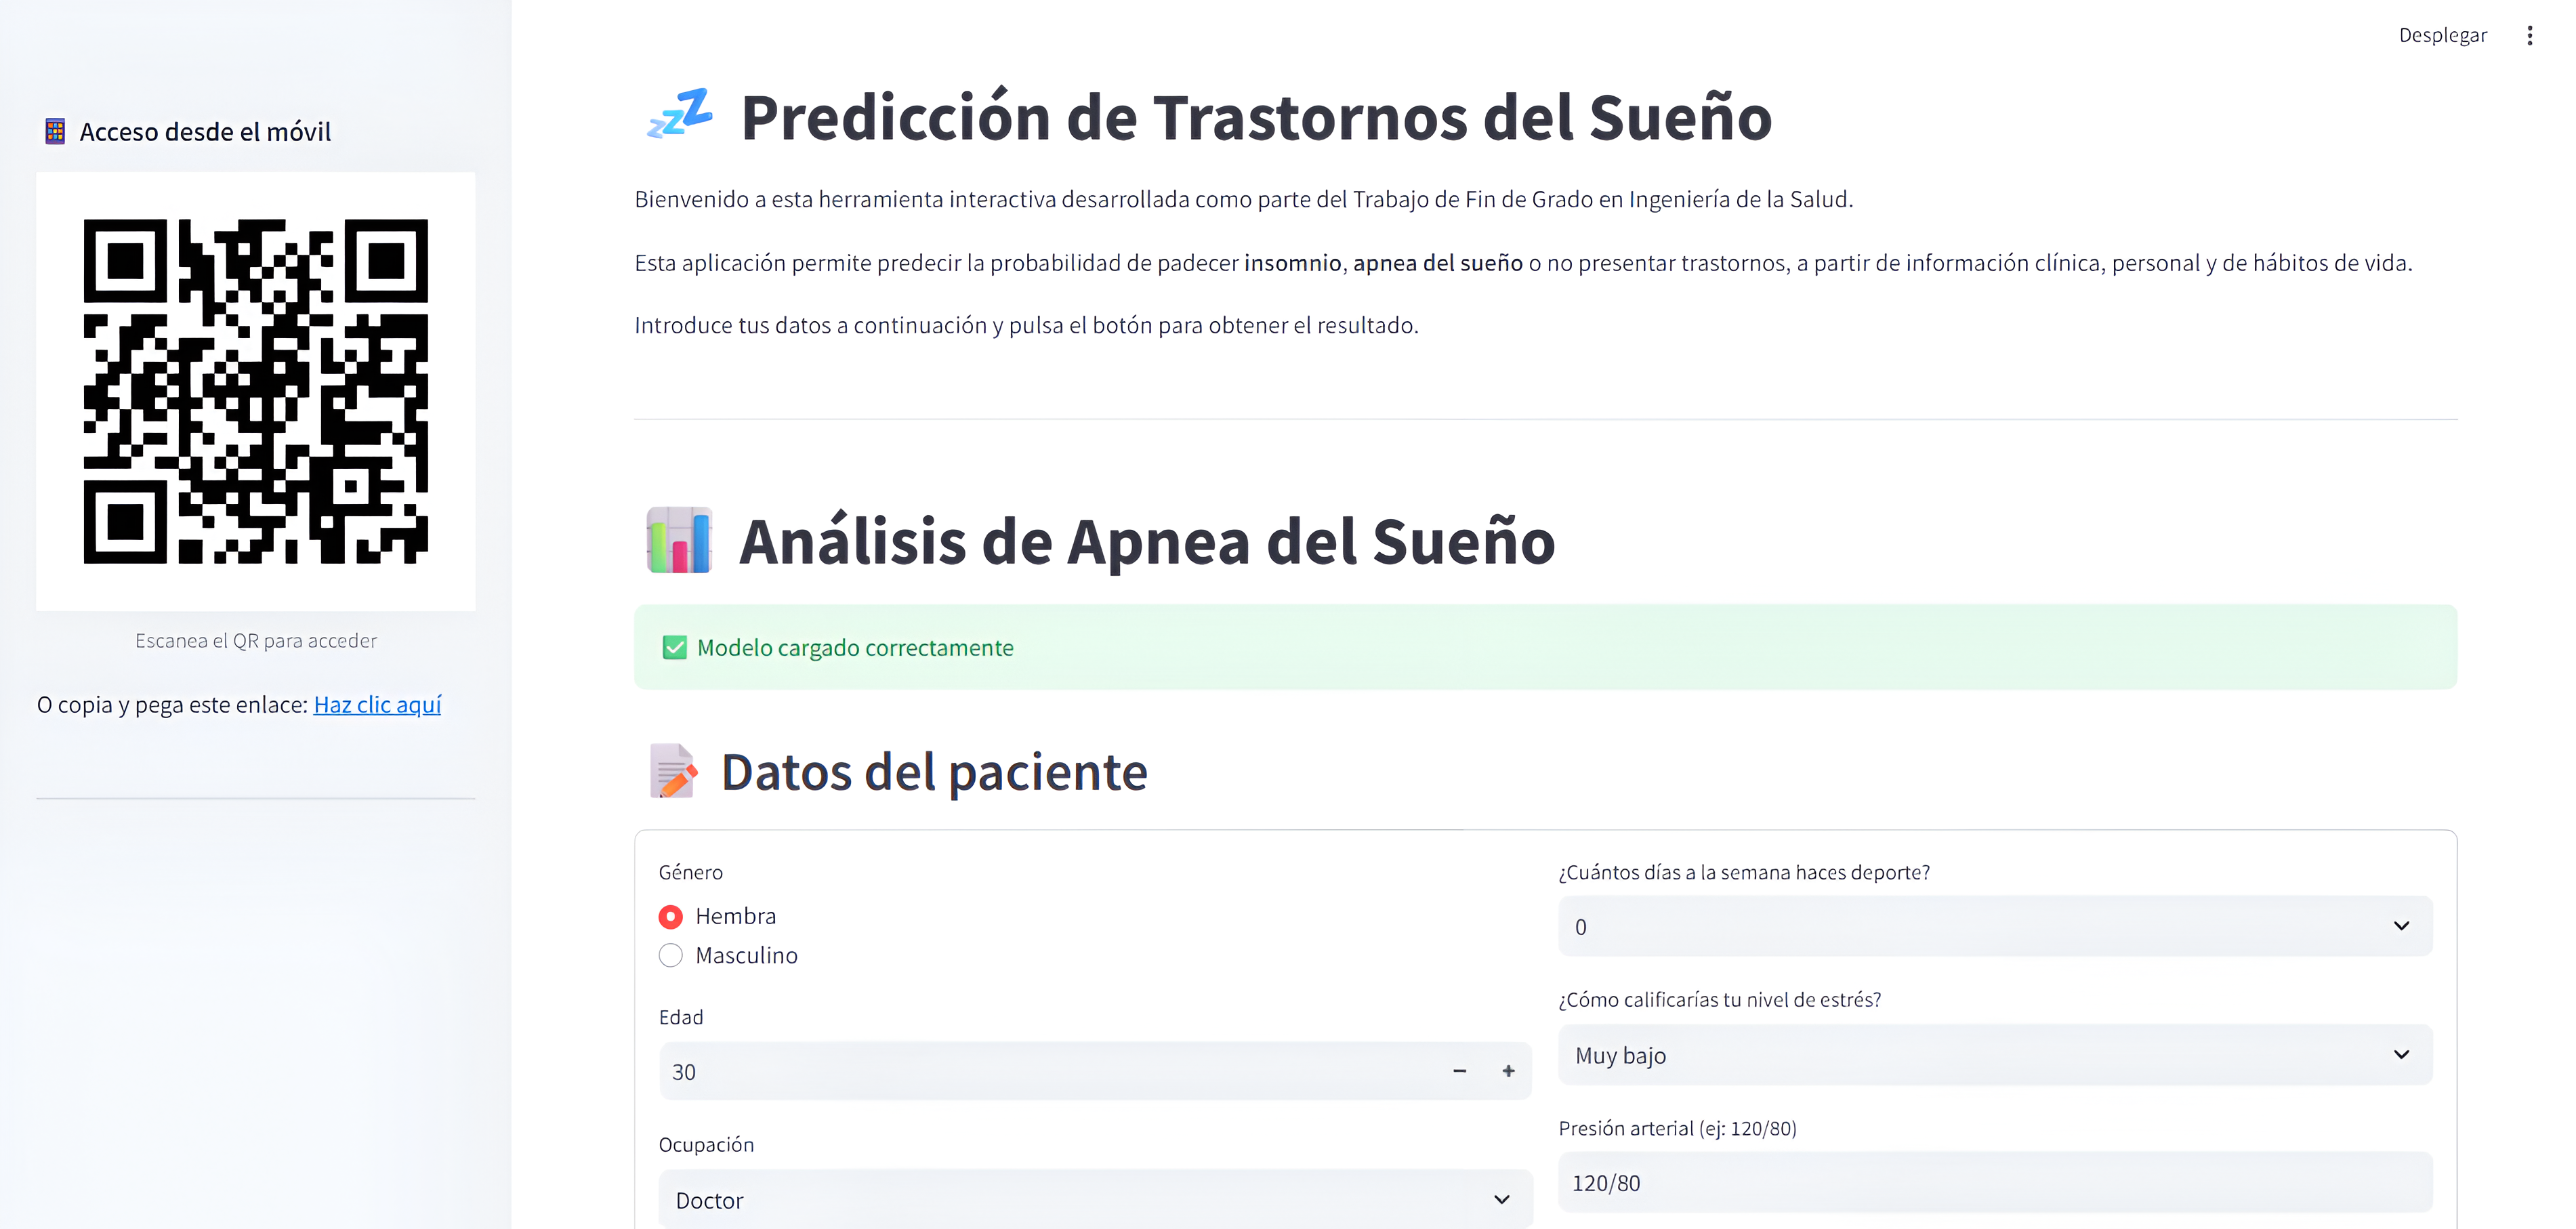
\includegraphics[width=0.9\linewidth]{img/interfazApp.png}
        \caption{Vista inicial de la aplicación en Streamlit Cloud.}
        \label{fig:inicio}
    \end{figure}

\subsection{Introducción de datos}

    El usuario completa el formulario con su edad, género, ocupación, calidad del sueño, frecuencia cardíaca, presión arterial, pasos diarios, etc. El sistema valida automáticamente que los campos obligatorios estén correctamente rellenados y que los datos introducidos tengan un formato válido (por ejemplo, la presión arterial debe seguir el formato '120/80'). Cualquier error impide avanzar a la siguiente fase, asegurando la consistencia de entrada.



    \begin{figure}[H]
        \centering
        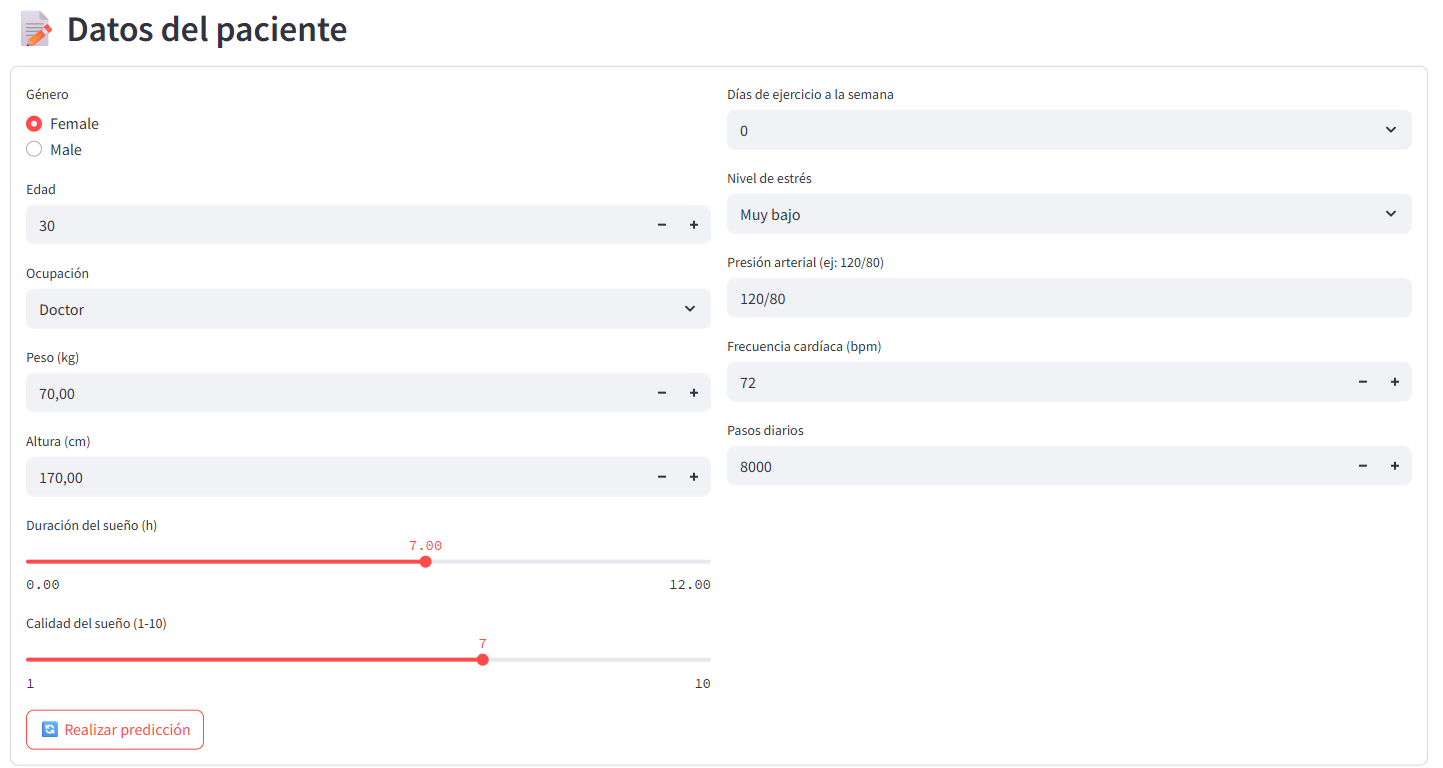
\includegraphics[width=0.9\linewidth]{img/formularioApp.png}
        \caption{Formulario con datos clínicos y de estilo de vida.}
        \label{fig:formulario}
    \end{figure}

\subsection{Generación de predicción}
Tras completar el formulario, se realiza una predicción automática del posible trastorno del sueño. El sistema utiliza un modelo Random Forest calibrado y previamente entrenado, que clasifica al paciente en una de las siguientes categorías:

\begin{itemize}
    \item Insomnio
    \item Apnea del sueño
    \item Ausencia de trastorno (\texttt{None})
\end{itemize}

    \begin{figure}[H]
        \centering
        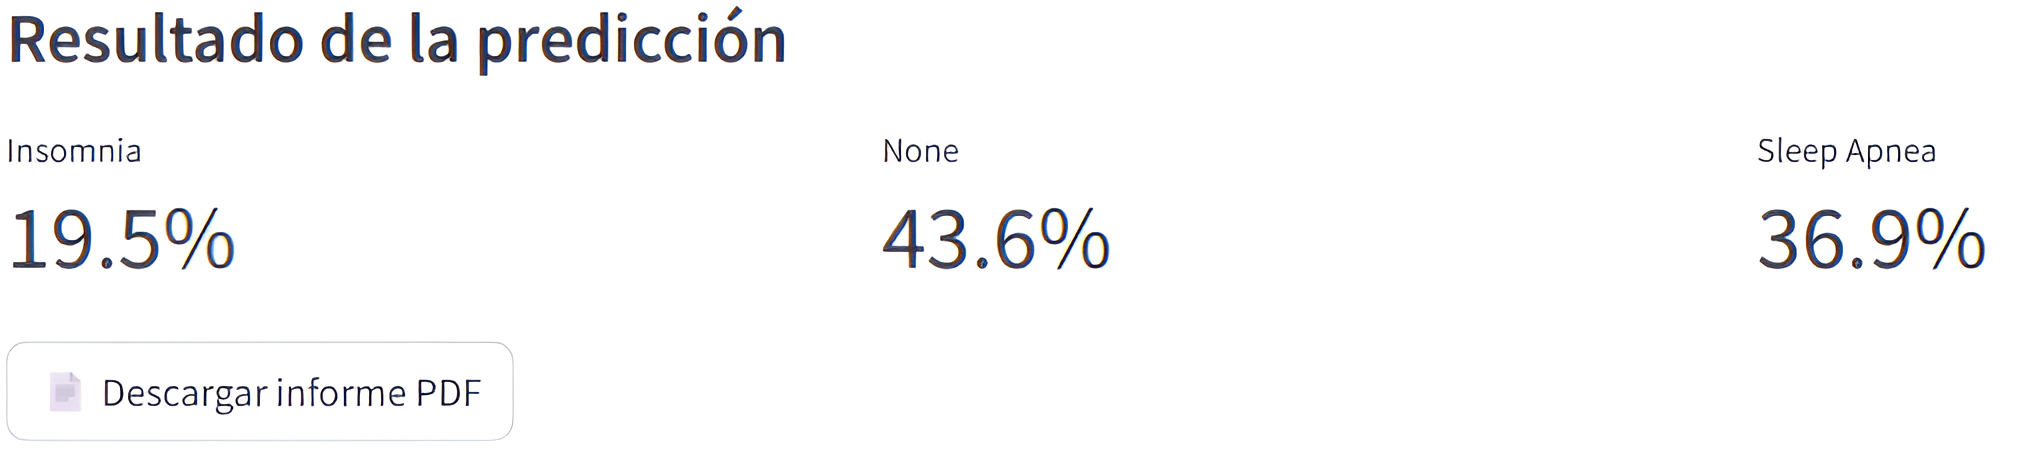
\includegraphics[width=0.9\linewidth]{img/resultadoPredd.png}
        \caption{Resultado de la predicción con las probabilidades asociadas.}
        \label{fig:prediccion}
    \end{figure}
    
\subsection{Explicación de la predicción} 
Se muestra un gráfico de interpretabilidad basado en SHAP (SHapley Additive exPlanations) que indica la influencia relativa de cada variable sobre la predicción realizada. Esta visualización ayuda al profesional a comprender qué factores han motivado la clasificación del modelo.
La aplicación permite interpretar los resultados mediante gráficos SHAP (SHapley Additive exPlanations), una técnica que descompone la predicción del modelo en contribuciones individuales de cada variable.

En primer lugar, se proporciona una explicación individualizada para el caso introducido, mostrando qué variables han influido de forma positiva o negativa en el diagnóstico sugerido. Este análisis ayuda al profesional a entender el razonamiento detrás de la predicción concreta para un paciente específico.

    \begin{figure}[H]
        \centering
        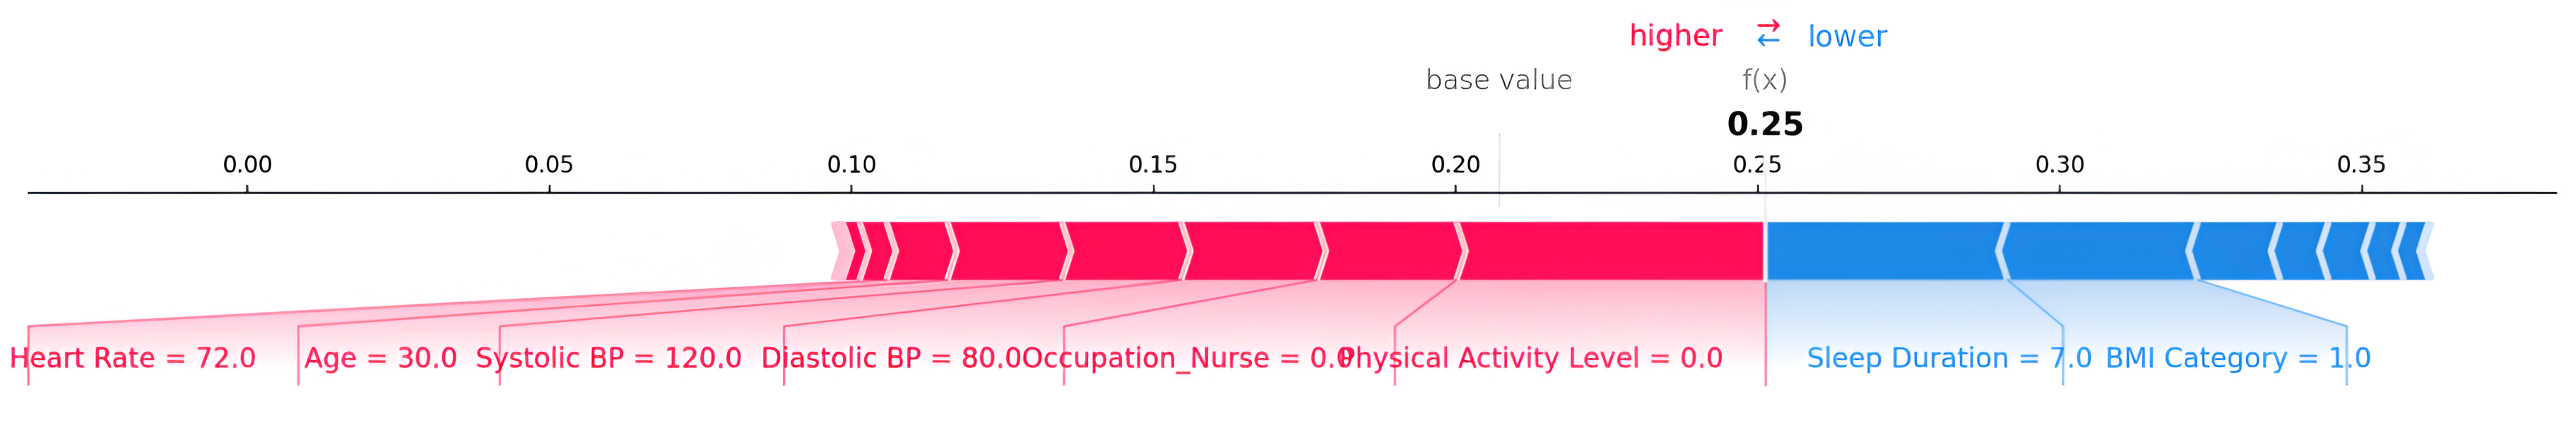
\includegraphics[width=0.95\textwidth]{img/explicacIndividual.png}
        \caption{Interpretación SHAP individual de un caso clínico simulado.}
        \label{fig:shap-individual}
    \end{figure}

Además, el sistema incluye una visualización global que muestra, en promedio, qué variables tienen mayor peso en las decisiones del modelo para todos los casos. Esta vista general es útil para identificar los factores clínicos más relevantes en la predicción automática.

\begin{figure}[H]
    \centering
    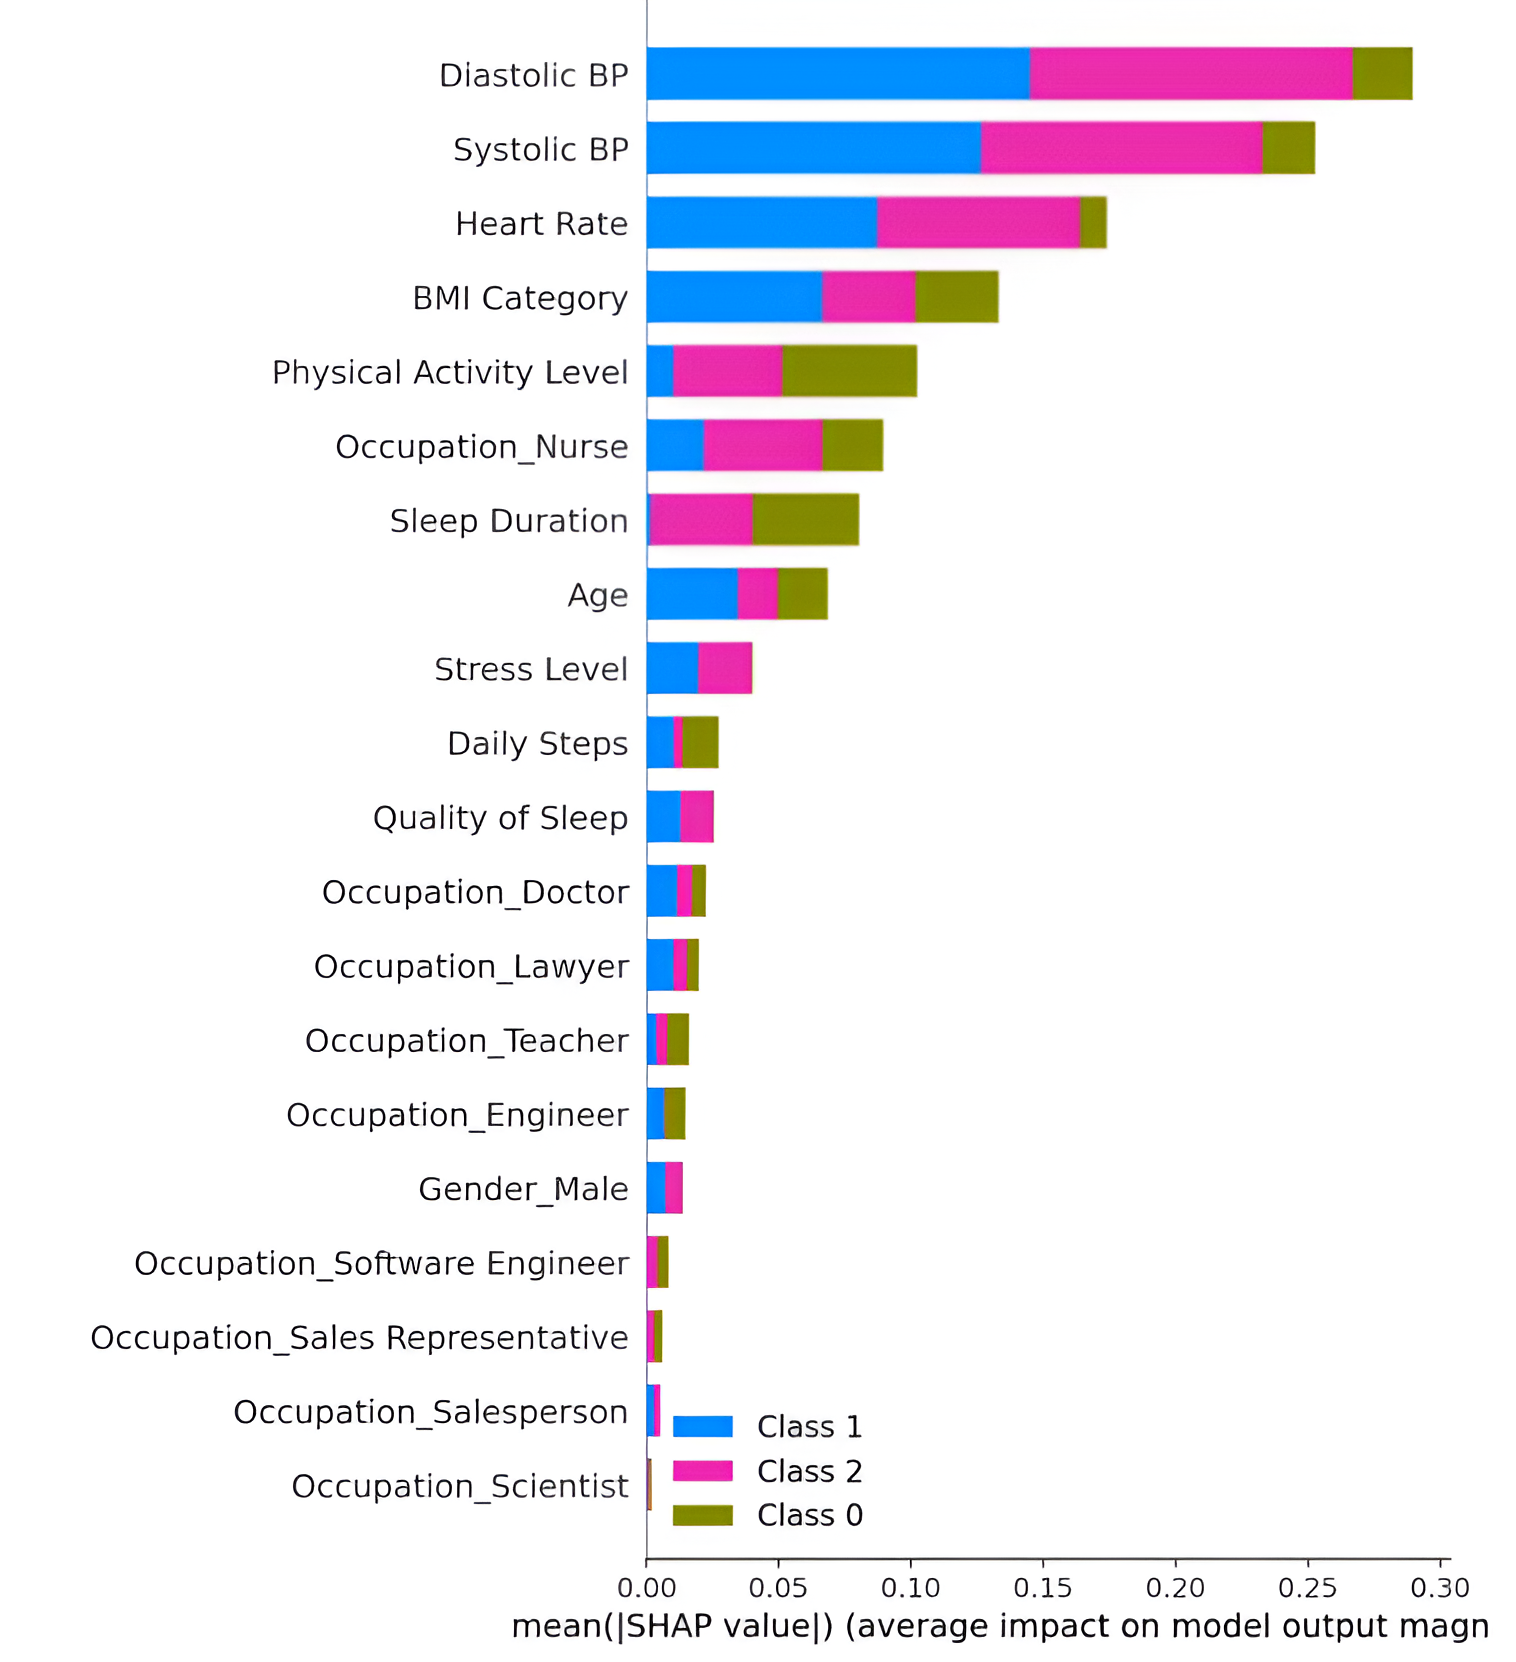
\includegraphics[width=0.85\textwidth]{img/SHAP.png}
    \caption{Importancia global de las variables según el modelo (gráfico SHAP).}
    \label{fig:shap-global}
\end{figure}

\subsection{Generación del informe} 
El sistema permite descargar un informe clínico personalizado en formato PDF que incluye:

\begin{itemize}
    \item Datos introducidos
    \item Clase predicha
    \item Probabilidades por clase
    \item Explicación visual
\end{itemize}
El informe puede guardarse localmente o imprimirse para su incorporación al historial del paciente, facilitando su uso como documento complementario en procesos de cribado o seguimiento clínico.


    \begin{figure}[H]
        \centering
        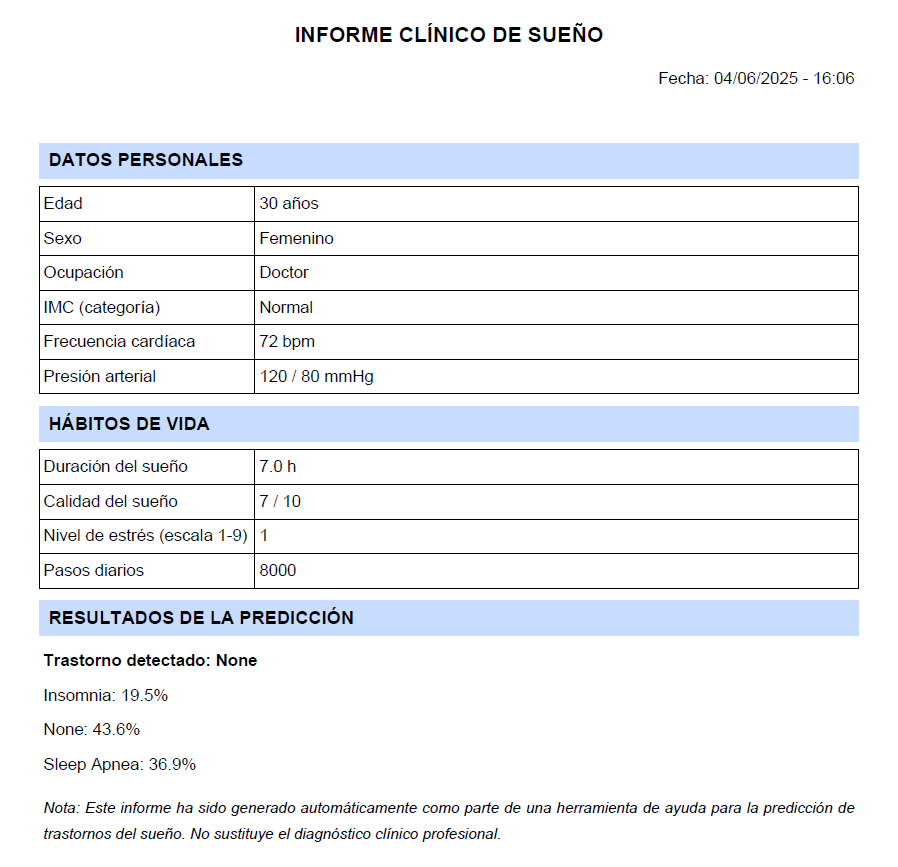
\includegraphics[width=1\linewidth]{img/pdfApp.png}
        \caption{Vista previa del informe PDF generado.}
        \label{fig:pdf}
    \end{figure}
    
Durante el desarrollo se ha verificado que la aplicación funciona de forma fluida y estable desde el punto de vista técnico, permitiendo una interacción clara con el usuario, la visualización de resultados interpretables y la generación automática de informes PDF. Aunque existen aspectos mejorables en cuanto al comportamiento predictivo del modelo, esta herramienta representa una base funcional sólida sobre la que podrían construirse futuras versiones con validación clínica ampliada.
